\chapter{Análisis de los resultados obtenidos}\label{cp: results}
El algoritmo planteado fue entrenado con el dataset completo sin obtener resultados durante pocas épocas dado el elevado tiempo de entrenamiento por época. La precisión en entrenamiento no aumentaba con el paso de las épocas y se decidió reducir la complejidad del problema. Para ello, se entrenó el algoritmo con dos grabaciones de audio y se validó para una única grabación de audio. El algoritmo se entrenó con las siguientes características:
\begin{itemize}
	\item \textbf{Tamaño de batch}\arrowTikz{0}32
	\item \textbf{Número de \glspl{FFT}}
	\begin{itemize}
		\item Entrenamiento\arrowTikz{0}63132
		\item Validación\arrowTikz{0}4068
	\end{itemize}
	\item \textbf{Número de épocas}\arrowTikz{0}2000\footnote{El entrenamiento se paró en 1390 al comprobar que los resultados empeoraban}
	\item \textbf{Tasa de aprendizaje}\arrowTikz{0}Variable en el tiempo como muestra la gráfica \ref{fig: learning_rate}
\end{itemize}

\begin{figure}[h!]
	\centering
	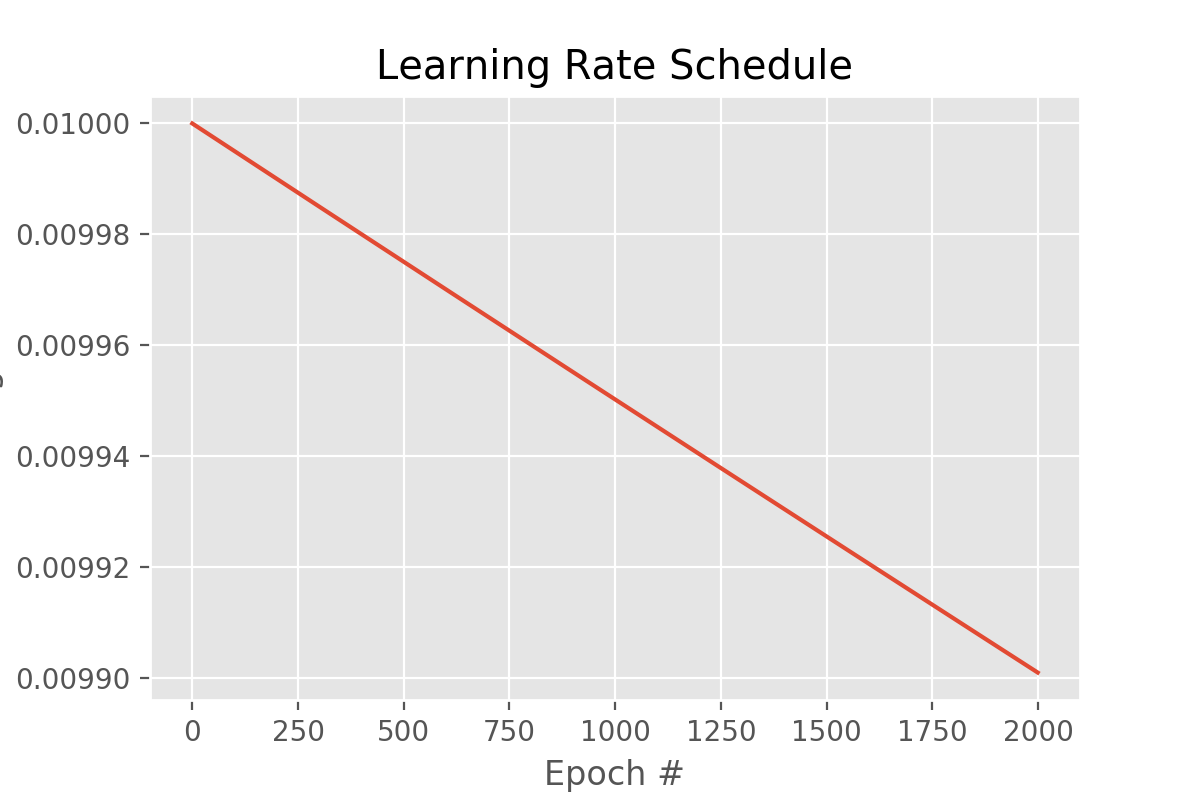
\includegraphics[width=0.75\columnwidth]{figures/Learning_rate_schedule}
	\caption{Variación de la tasa de aprendizaje con las épocas}
	\label{fig: learning_rate}
\end{figure}

Entrenado con esta configuración, el tiempo de entrenamiento por época es de 36 segundos con $\approx 569\mu$s por batch en una tarjeta gráfica \gls{AMD} Radeon Rx570 mediante el \gls{framework} \gls{ROCm}. 

Los resultados obtenidos distan mucho de un correcto funcionamiento. La precisión en entrenamiento se estabiliza en torno al 5\% y la precisión en validación llega al 2\% y decae hasta el 1\% claro síntoma de \textbf{overfitting} a pesar de tener una pobre precisión en entrenamiento.

\begin{figure}[h!]
	\centering
	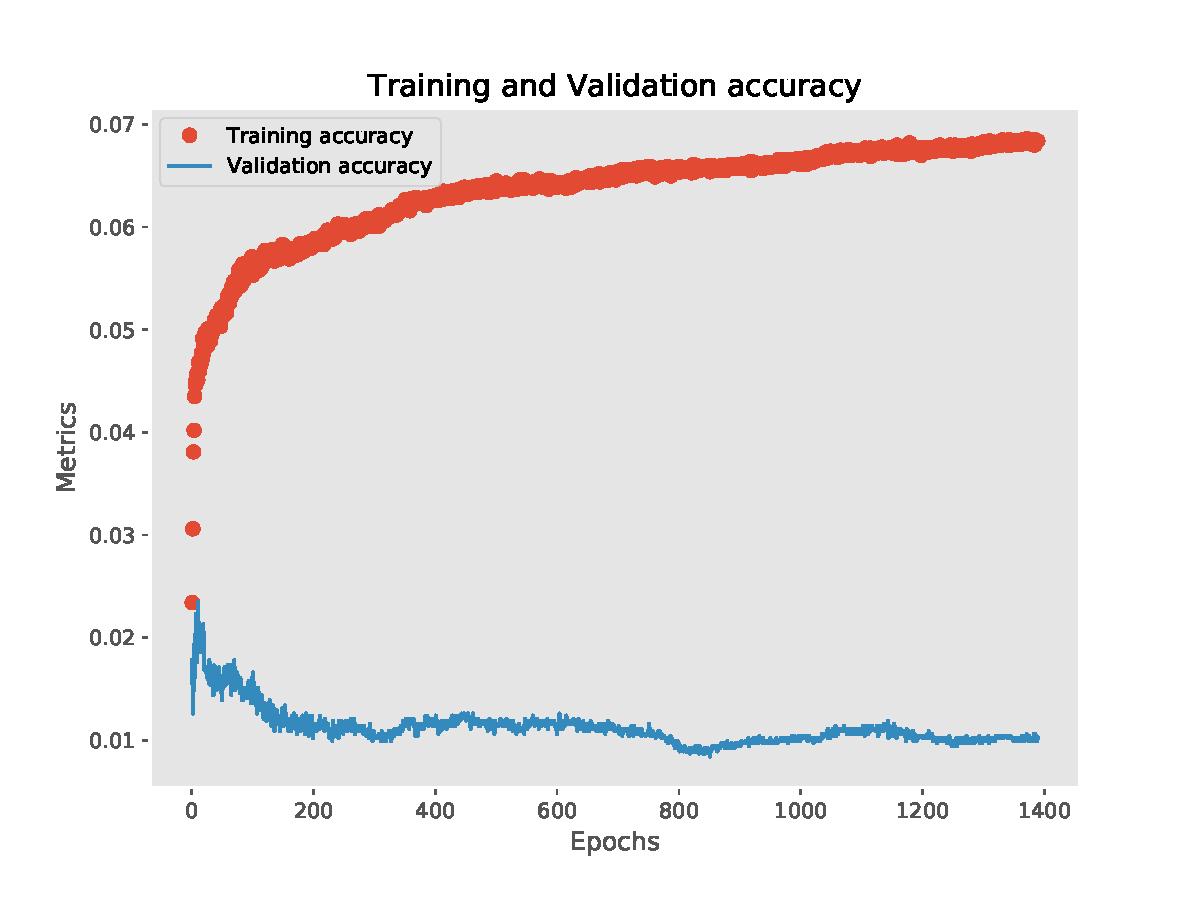
\includegraphics[width=0.75\columnwidth]{figures/one_to_one_results_acc.pdf}
	\caption{Precisión en entrenamiento y validación}
	\label{fig: results_acc}
\end{figure}
\begin{figure}[t!]
	\centering
	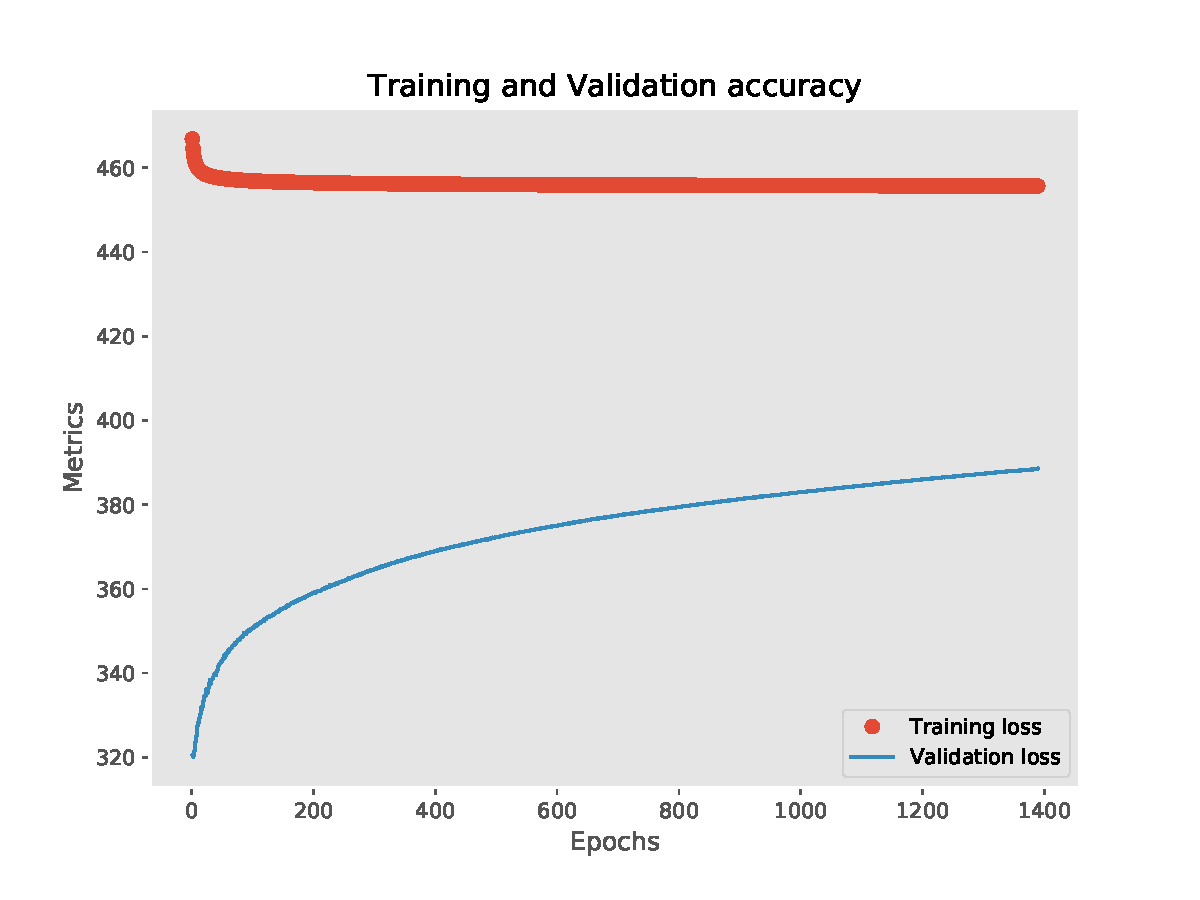
\includegraphics[width=0.75\columnwidth]{figures/one_to_one_results_loss.pdf}
	\caption{Pérdidas en entrenamiento y validación}
	\label{fig: results_loss}
\end{figure}

En las figuras \ref{fig: results_acc} y \ref{fig: results_loss} se puede ver las comparativas de pérdidas y precisión para entrenamiento y validación, respectivamente. En la gráficas se aprecia el claro overfitting. Algo a destacar es la lenta memorización de datos porque una red tan grande debería ser capaz de memorizar los datos de entrenamiento. Como se aprecia la precisión en entrenamiento no llega a una asíntota de modo que, idealmente debería continuar memorizando los datos con el paso de las épocas.